\documentclass[aspectratio=169,11pt]{beamer}
\usetheme{default}
\usecolortheme{default}
\usepackage[T1]{fontenc}
\usepackage{lmodern}
\usepackage{pgfplots}\pgfplotsset{compat=1.18}
\usepackage{booktabs,array}

% DreamLab brand
\definecolor{teal0}{RGB}{0,128,128}
\definecolor{burnt}{RGB}{204,85,0}
\definecolor{ink}{RGB}{38,42,46}
\definecolor{paper}{RGB}{250,249,246}
\definecolor{grayln}{RGB}{200,200,200}
\definecolor{softgreen}{RGB}{46,139,87}

\setbeamercolor{background canvas}{bg=paper}
\setbeamercolor{normal text}{fg=ink}
\setbeamercolor{frametitle}{fg=teal0}
\setbeamercolor{title}{fg=teal0}
\setbeamercolor{subtitle}{fg=burnt}
\setbeamercolor{author}{fg=ink}
\setbeamercolor{date}{fg=ink}
\setbeamercolor{item}{fg=teal0}
\setbeamercolor{block title}{fg=paper,bg=teal0}
\setbeamercolor{block body}{fg=ink,bg=paper}
\setbeamerfont{frametitle}{series=\bfseries,size=\Large}
\setbeamerfont{title}{series=\bfseries,size=\huge}
\setbeamertemplate{navigation symbols}{}
\setbeamertemplate{footline}{%
  \hfill\textcolor{grayln}{\tiny DreamLab AI \textbullet\ Ontology Eval 2026\quad\insertframenumber}\hspace{6pt}\vspace{4pt}%
}

\pgfplotsset{
  every axis/.append style={font=\small,axis line style={grayln},tick style={grayln},
    grid=major,major grid style={grayln!40}},
  augstyle/.style={fill=teal0,draw=teal0!60},
  ctlstyle/.style={fill=burnt,draw=burnt!60},
}

\title{Can a Local Model Beat the Frontier?}
\subtitle{Ontology-Grounded DiffusionGemma vs.\ Bare Cloud Models}
\author{Dr John O'Hare \\ \small DreamLab AI}
\date{June 2026}

\begin{document}

% SLIDE 1: TITLE
\begin{frame}[plain]
\maketitle
\end{frame}

% SLIDE 2: THE QUESTION
\begin{frame}{One Question}
\Large
\begin{center}
Can a \textcolor{softgreen}{\textbf{local model}} running on one GPU,\\[6pt]
grounded in a \textcolor{teal0}{\textbf{formal knowledge graph}},\\[6pt]
match \textcolor{burnt}{\textbf{frontier cloud models}} on domain recall?
\end{center}
\vfill
\normalsize
\textcolor{grayln}{7 models \textbullet\ 672 isolated runs \textbullet\ 16 KG-oracle questions \textbullet\ deterministic grading}
\end{frame}

% SLIDE 3: HEADLINE RESULT
\begin{frame}{Headline: Local + Ontology Beats Every Frontier Bare}
\centering
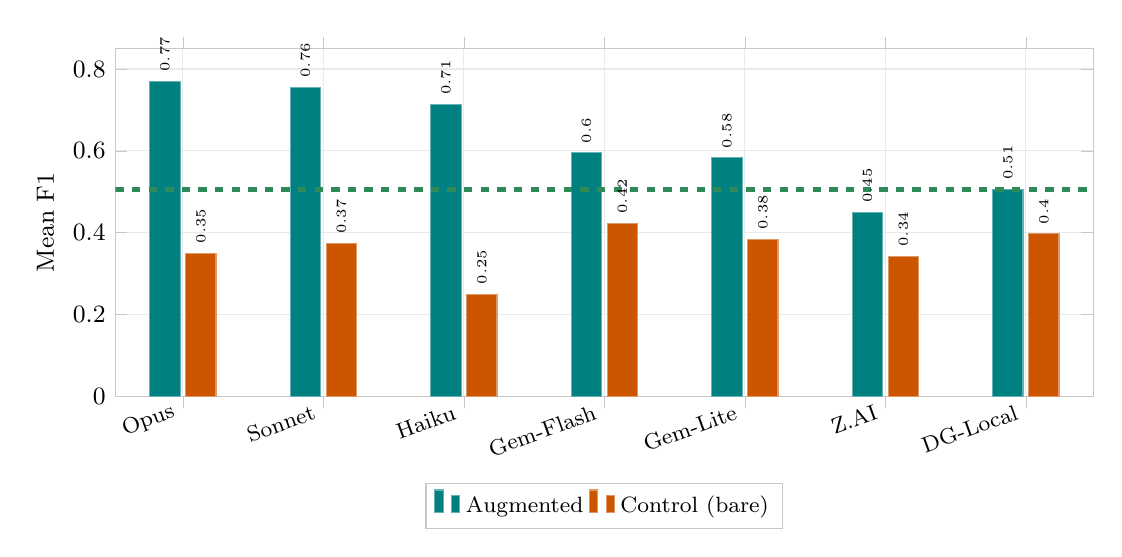
\begin{tikzpicture}
\begin{axis}[ybar,width=14cm,height=6cm,bar width=11pt,ymin=0,ymax=0.85,
  ylabel={Mean F1},
  symbolic x coords={Opus,Sonnet,Haiku,Gem-Flash,Gem-Lite,Z.AI,DG-Local},
  xtick=data,x tick label style={rotate=20,anchor=east,font=\footnotesize},
  enlarge x limits=0.08,
  legend style={at={(0.5,-0.25)},anchor=north,legend columns=3,draw=grayln,font=\footnotesize},
  nodes near coords,nodes near coords style={font=\tiny,rotate=90,anchor=west}]
\addplot[augstyle] coordinates {(Opus,0.770) (Sonnet,0.755) (Haiku,0.713) (Gem-Flash,0.595) (Gem-Lite,0.583) (Z.AI,0.449) (DG-Local,0.505)};
\addplot[ctlstyle] coordinates {(Opus,0.350) (Sonnet,0.373) (Haiku,0.250) (Gem-Flash,0.423) (Gem-Lite,0.384) (Z.AI,0.342) (DG-Local,0.397)};
\draw[softgreen,line width=1.8pt,dashed] ({rel axis cs:0,0}|-{axis cs:Opus,0.505}) -- ({rel axis cs:1,0}|-{axis cs:Opus,0.505});
\legend{Augmented,Control (bare),DG+ontology (0.505)}
\end{axis}\end{tikzpicture}

\vspace{-2mm}
{\small\textcolor{softgreen}{\textbf{Dashed line}} = local DiffusionGemma + ontology. Every frontier bare score falls below it.}
\end{frame}

% SLIDE 4: THE NUMBERS
\begin{frame}{Full Results}
\centering
\small
\begin{tabular}{lcccc}
\toprule
Model & AUG F1 & Bare F1 & $\Delta$ & Halluc drop \\
\midrule
Opus 4.8 & \textbf{0.770} & 0.350 & \textcolor{burnt}{+0.420} & \textcolor{teal0}{--0.529} \\
Sonnet 4.6 & 0.755 & 0.373 & \textcolor{burnt}{+0.382} & \textcolor{teal0}{--0.480} \\
Haiku 4.5 & 0.713 & 0.250 & \textcolor{burnt}{+0.463} & \textcolor{teal0}{--0.608} \\
Gemini 3.5 Flash & 0.595 & 0.423 & \textcolor{burnt}{+0.172} & \textcolor{teal0}{--0.210} \\
Gemini 2.5 Flash Lite & 0.583 & 0.384 & \textcolor{burnt}{+0.199} & \textcolor{teal0}{--0.232} \\
Z.AI (GLM-4.6) & 0.449 & 0.342 & \textcolor{burnt}{+0.108} & \textcolor{teal0}{--0.206} \\
\midrule
\textbf{DiffusionGemma (local)} & \textbf{0.505} & 0.397 & \textcolor{burnt}{+0.108} & \textcolor{teal0}{--0.199} \\
\bottomrule
\end{tabular}

\vspace{4mm}
\textbf{Every model benefits. Hallucination drops across the board.}
\end{frame}

% SLIDE 5: BY QUESTION TYPE
\begin{frame}{Where Grounding Helps Most}
\centering
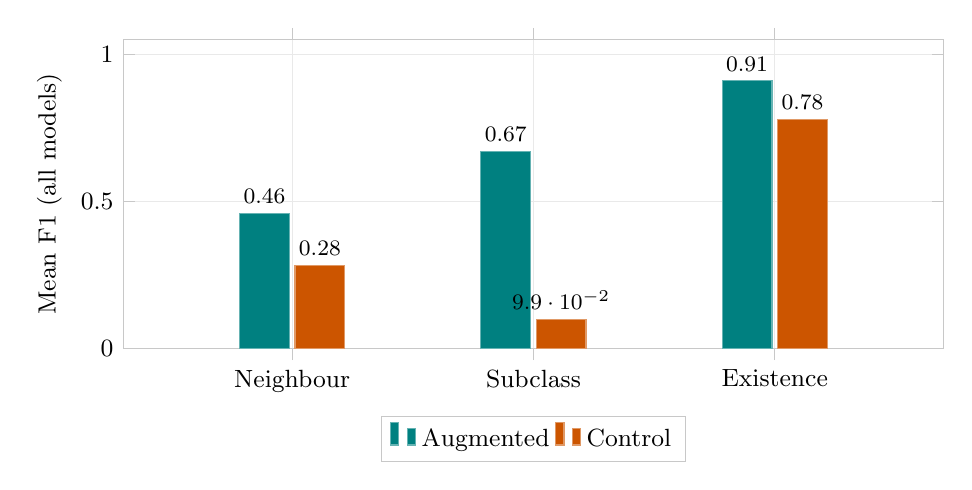
\begin{tikzpicture}
\begin{axis}[ybar,width=12cm,height=5.5cm,bar width=18pt,ymin=0,ymax=1.05,
  ylabel={Mean F1 (all models)},symbolic x coords={Neighbour,Subclass,Existence},xtick=data,
  enlarge x limits=0.35,legend style={at={(0.5,-0.22)},anchor=north,legend columns=2,draw=grayln},
  nodes near coords,nodes near coords style={font=\footnotesize}]
\addplot[augstyle] coordinates {(Neighbour,0.458) (Subclass,0.671) (Existence,0.910)};
\addplot[ctlstyle] coordinates {(Neighbour,0.281) (Subclass,0.099) (Existence,0.778)};
\legend{Augmented,Control}
\end{axis}\end{tikzpicture}

\vspace{-2mm}
{\small \textbf{Subclass}: 6.8$\times$ improvement. Models have near-zero parametric knowledge of ontology hierarchies.}
\end{frame}

% SLIDE 6: HALLUCINATION
\begin{frame}{Hallucination Halves with Grounding}
\centering
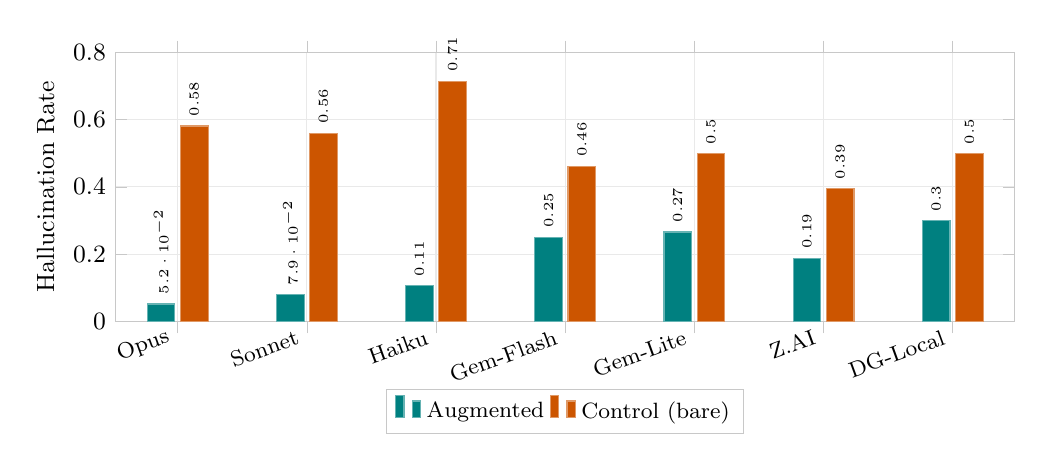
\begin{tikzpicture}
\begin{axis}[ybar,width=13cm,height=5cm,bar width=10pt,ymin=0,ymax=0.8,
  ylabel={Hallucination Rate},
  symbolic x coords={Opus,Sonnet,Haiku,Gem-Flash,Gem-Lite,Z.AI,DG-Local},
  xtick=data,x tick label style={rotate=20,anchor=east,font=\footnotesize},
  enlarge x limits=0.08,
  legend style={at={(0.5,-0.25)},anchor=north,legend columns=2,draw=grayln,font=\footnotesize},
  nodes near coords,nodes near coords style={font=\tiny,rotate=90,anchor=west}]
\addplot[augstyle] coordinates {(Opus,0.052) (Sonnet,0.079) (Haiku,0.106) (Gem-Flash,0.250) (Gem-Lite,0.266) (Z.AI,0.188) (DG-Local,0.299)};
\addplot[ctlstyle] coordinates {(Opus,0.581) (Sonnet,0.559) (Haiku,0.714) (Gem-Flash,0.460) (Gem-Lite,0.498) (Z.AI,0.394) (DG-Local,0.498)};
\legend{Augmented,Control (bare)}
\end{axis}\end{tikzpicture}

\vspace{-1mm}
{\small Overall: 0.529 $\to$ 0.177. KG grounding provides verifiable facts, not plausible guesses.}
\end{frame}

% SLIDE 7: COST / PRIVACY
\begin{frame}{Cost, Privacy, and Data Sovereignty}
\centering
\small
\begin{tabular}{lccc}
\toprule
& \textbf{DG Local + Ontology} & \textbf{Frontier AUG} & \textbf{Frontier Bare} \\
\midrule
F1 (best) & 0.505 & \textbf{0.770} (Opus) & 0.423 (Gem-Flash) \\
Data leaves org? & \textcolor{softgreen}{\textbf{No}} & Yes & Yes \\
Per-query cost & \textcolor{softgreen}{\textbf{\$0*}} & \$0.01--0.08 & \$0.002--0.04 \\
Latency & \textcolor{softgreen}{\textbf{2--4\,s}} & 15--50\,s & 5--15\,s \\
GDPR-compliant? & \textcolor{softgreen}{\textbf{Yes}} & Depends & Depends \\
\bottomrule
\end{tabular}

\vspace{5mm}
\begin{columns}
\begin{column}{0.5\textwidth}
\textbf{For regulated industries:}
\begin{itemize}
\item Zero data exfiltration
\item Predictable, flat cost
\item Sub-second KG lookup
\end{itemize}
\end{column}
\begin{column}{0.5\textwidth}
\textbf{Ontology condense cost:}
\begin{itemize}
\item One-off: 6h for 7{,}445 classes
\item Re-index only when KG changes
\item Per-query: sub-ms cache read
\end{itemize}
\end{column}
\end{columns}

\vspace{2mm}
{\tiny *Amortised electricity/hardware only.}
\end{frame}

% SLIDE 8: CAVEATS
\begin{frame}{Important Caveats}
\begin{enumerate}
\item \textbf{Not like-for-like.} Local model receives KG triples; frontier models get only the
      question. If frontier models were also grounded, they score much higher (Opus AUG: 0.770).

\item \textbf{Frontier models gain more from grounding.} Claude +0.38--0.46 vs.\ DiffusionGemma
      +0.108. The ontology is a \emph{capability multiplier}; it scales with the base model.

\item \textbf{DG's own lift is modest.} +0.108 F1. Its strength is a surprisingly competitive
      bare score (0.397), not exceptional ontology use.

\item \textbf{Performance varies by type.} DG excels on existence (0.875) but struggles on
      neighbour recall (0.323) due to the 256-token block decode limit.

\item \textbf{Domain-specific only.} Results measure KG fidelity, not general QA.
\end{enumerate}
\end{frame}

% SLIDE 9: KEY TAKEAWAYS
\begin{frame}{Key Takeaways}
\Large
\begin{enumerate}
\item \textcolor{teal0}{\textbf{Ontology grounding works.}} Universally, across 7 models.\\
      {\normalsize +0.265 F1, hallucination halved}

\vspace{4mm}
\item \textcolor{softgreen}{\textbf{Local + ontology $>$ frontier bare.}} For domain recall.\\
      {\normalsize DiffusionGemma 0.505 beats Opus bare 0.350}

\vspace{4mm}
\item \textcolor{burnt}{\textbf{Data sovereignty without sacrificing accuracy.}}\\
      {\normalsize Zero API cost, zero data exfiltration, GDPR-ready}
\end{enumerate}

\vfill
\begin{center}
{\small\textcolor{grayln}{672 runs \textbullet\ 7 models \textbullet\ 7{,}445 OWL classes \textbullet\ deterministic grading}}\\[4pt]
{\footnotesize\textcolor{teal0}{DreamLab AI} \textbullet\ Dr John O'Hare \textbullet\ \texttt{ontology-augment} (PRD-020)}
\end{center}
\end{frame}

\end{document}
